\chapter{Structural Concepts and Architecture}

\section*{}
An Electronic Health Record can be defined as the set of some essential healthcare services. In this section, we will describe the services which we consider the most important ones.

\section{Patient Summary} \label{sec:pat_sum}

The Patient Summary (PS)~\citep{EPSOS_PS} is a set of information that allows an healthcare professional to have a quick and easy overview over a patient, used in the epSOS project. A similar concept is used in the England's National Health Service, called Summary Care Records. Although the name may vary, the concept is practically the same and stands as an electronic record that will give healthcare staff faster, easier access to essential information about a patient, to help provide safe treatment in an emergency, generally~\citep{Service2010}.

The epSOS Patient Summary contains the following data:
\begin{itemize}
\item Demographic information (e.g. name, birth date, gender);
\item Most important clinical patient data (e.g. allergies, current medical problems, or major surgical procedures during the last six months);
\item Current medication including all prescribed medicines;
\item Meta-data about the Patient Summary itself (e.g. when and by whom was created or modified).
\end{itemize}

The clinical data included may vary a little bit but, in general terms, is very similar to the set stated above. 

The benefits of the existence of a Patient Summary are not very consensual. In general terms, the advantages announced are:
\begin{itemize}
\item Improved information flow between patient and staff;
\item Better and more accurate treatment in emergency situations;
\item Quicker and easier access to essential information;
\item Easier to allow the patient to check its own PS.
\end{itemize}

In fact, it is possible to point out two completely different case studies, in terms of acceptance and success: England and Scotland. 

In England, several articles~\citep{Anderson2010, Coiera2011, Greenhalgh2010} had been written expressing concerns and doubts about the concept, arguing that the Summary Care Record (in England) should be abandoned "for reasons of safety, functionality, clinical autonomy, patient privacy, and human rights"~\citep{Anderson2010}, stated Ross Anderson. Anderson justifies his critical saying that the data coming from multiple sources, for which there is no responsible, will create a poor and dangerously incomplete summary. Moreover, a final report~\citep{Stramer2010} of an independent evaluation of the Summary Care Record programme concluded that there is limited evidence that the SCR programme had so far achieved the benefits set out. Despite of stating an evidence of improved quality in some consultations, particularly those which involved medication decisions and a probably reduce of rare but important medication errors, the commission was not able neither to find evidence of reduction in onward referral nor to evaluate the impact on the satisfaction of patients. Although, the report defends that the SCR was particularly useful in patients unable to communicate or advocate for themselves. On the other hand, Mark Walport advocates~\citep{Walport2010} that "good information technology has the capacity to be transformational" insisting on the idea of quicker access to more reliable information that should help the treatment.

The Scottish case appears to gather more consensus and positive feedback. A study of Gartner Industry Research stated~\citep{Research2007} that the Emergency Care Summary (ECS), how it is called in Scotland, is a success because it met a specific business need. Also, it advocates that the clinician buy-in was achieved by involving the clinicians in the definition of ECS data and designing the security and access protocol for it as well as there was "training out-of-hours staff to use ECS appropriately" which was identified as a critical factor too. Another study~\citep{Jones2008} on the ECS reported an estimated volume of 5.1 million patient records created from the GP practices and 1.3 million of accesses to them, in 2008.

\section{Personal Health Record}

A Personal Health Record is a system whereby individuals can "access, manage and share their health information, and that of others for whom they are authorized, in a private, secure, and confidential environment"~\citep{Health2003}. As it is reported by some articles~\citep{Tang2006,Tang2009}, the approach of the system might differ from being a totally isolated one till being integrated with the national healthcare system. Also, there is a lot of studies~\cite{Tang2009,Pagliari2007,Detmer2008, Fricton2008} about the benefits that those systems can bring:
\begin{itemize}
\item quality, completeness, depth, and accessibility of health information provided by patients;
\item self management support - e.g. care plans, graphing of symptoms, passive biofeedback, tailored instructive or motivational feedback, decision aids, or reminders;
\item communication between patients and providers;
\item access to patients' health knowledge;
\item portability of clinical records and other personal health information;
\item links to static or interactive information about illness, treatments, or self care;
\item capture of symptom or health behaviour data by self report or objective monitoring through electronic devices.
\end{itemize}

This kind of system represents a new paradigm in which the patients have the central power about the information about himself~\citep{Ball2007}. Also, some new visions appeared, extracting the maximum value of the information inserted by the individual. For instance, how that information can be used in a mobile context~\citep{Brief2010}.






\section{European Patients - Smart open Services (epSOS)} \label{sec:epsos}

The epSOS (European Patients - Smart open Services) is the main European electronic Health (eHealth) project created by European Commission and the partners. The main objective is to improve the health assistance to citizens who are abroad their own country. It aims to do so by implementing an interoperability platform, allowing different countries to exchange vital information. In that context, one health professional could access patient data from another country improving and précising the medical treatment~\citep{EpSOS}.

\subsection{Services and Standards}

The epSOS is based on a Services-oriented Architecture. It states that all services are passive, implemented with traditional Web Services with their interfaces based on the Web Service Description Language [W3C WSDL 1.1]. When we say that the services are passive, it means that every transaction must be initiated by the consumer of the information.
The key element of epSOS is the National Contact Point (NCP) and it stands as the only peer of contact for one determined country. In this sense, an NCP can serve both as a content provider when the request is made from other countries or as a gateway for an information request from that country, conveying that request to the target one.

The NCP is based on a set of Common Components and when connecting those components to the national infrastructure it is possible to offer the following end-user services: Consent Service, Patient and Order Services, eDispensation Service, Auditing Service.

\subsubsection{Consent Service}
epSOS states that the patient must consent and allow the sharing of his information between peers of the epSOS network. This consent is realized through the IHE Basic Patient Privacy Consents (BPPC) profile\footnote{Details: \url{http://wiki.ihe.net/index.php?title=Basic_Patient_Privacy_Consents}} and the patient's consent is given in the origin country.

\subsubsection{Patient and Order Services}
The Patient and Order Services are used to retrieve medical information when abroad of the patient's home country. The medical data is returned in the epSOS common format and is realized by the IHE Profile XCA\footnote{Details: \url{http://wiki.ihe.net/index.php?title=Cross-Community_Access}} Cross Gateway Query and Cross Gateway Retrieve. These documents are transmitted by web services exchanges and are complaints with the HL7 CDA Release 2.0 standard (see \ref{sec:hl7-cda}).

There are two type of documents to be exchanged: the `ePrescrition' and the `Patient Summary', both using epSOS specific CDA Level 1 and Level 3, respectively.

\subsubsection{eDispensation Service}

The eDispensation Service is required whenever it is necessary to update some medical data with some new information. In this context, one `eDispensation' document is dispatched from the actual country to the patient's home country, being formatted with HL7 CDA Level 3.

\subsubsection{Auditing Services}

The Auditing Services aim to guarantee that all that sensible information is only accessible by those who have that right. Thus, it defines some rules about how to achieve Auditing and Authentication using the IHE Profile Audit Trail and Node Authentication\footnote{Details: \url{http://wiki.ihe.net/index.php?title=Audit_Trail_and_Node_Authentication}}. 

\subsection{Security Aspects}
In terms of security, epSOS states some basic non-functional security requirements in order to guarantee that all transactions and data are reliable. Thus, epSOS must ensure: Identification, Authentication, Access Control, Non-repudiation, Data confidentiality, Data availability and Logging activities that impact security. Beyond these generic requirements, epSOS establishes some specific security requirements to be used in each country, dividing those into three levels:
\begin{itemize}
\item First level --- general epSOS as a whole (16 requirements);
\item Second level --- general NCP (34 requirements);
\item Third level --- national information infrastructure (9 requirements).
\end{itemize}

\subsection{Identification and Authentication}
\subsection{Semantic Issues}
epSOS is obviously an huge and complex project, presenting several challenges to manage and resolve. We know that each country has its own policy, classification tables, ontologies and so on. So, one of the most interesting challenges is how to handle this diversity, finding a common language which enables the communication and transcription of several local classifications and taxonomies, not to mention the country language itself. In order to address this problem, epSOS defines a set of semantic services which we describe next. 

\subsubsection{CDA's PPC in epSOS}
The CDA's PPC (Patient Care Coordination\footnote{Details: \url{http://wiki.ihe.net/index.php?title=Patient_Care_Coordination}}) was integrated in epSOS, creating a significant amount of data elements.

\subsubsection{epSOS Master Value Sets Catalogue}
The epSOS Master Value Sets Catalogue (MVC) contains all value sets used within epSOS system and CDA framework. The value sets were built based on several well-known code systems, like SNOMED CT, ICD-9, ICD-10, LOINC, ATC, HL7 and so forth. The epSOS MVC is distributed as an Excel file.

\subsubsection{epSOS Master Translation/Transcoding Catalogue}
The epSOS Master Translation/Transcoding Catalogue (MTC) is based on the epSOS MVC. It is made to fit the specific needs of a country and it is managed and updated its representatives. It is also provided as an Excel file.

\subsubsection{epSOS Ontology}
The epSOS Ontology aims to unify different terminologies that might be used in the future, providing a linguistic reference of the terms in the epSOS value sets.



\subsection{System Architecture}

epSOS architecture (described in Figure~\ref{fig:epsos-architecture}) was built with the objective of being enough flexible to allow integration with all kind of services existing inside the boundaries of each member state. The Figure~\ref{fig:epsos-architecture} presents the peer-to-peer connection between two countries. Also, it is possible to understand which components stay under the member state responsibility.

We will overview the main functions of each component in the next subsections, following a top-down approach.

\begin{figure}[t]
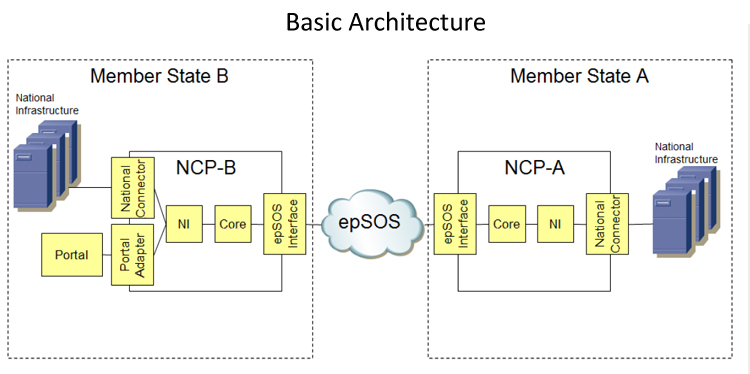
\includegraphics[width=1.0\textwidth]{basic-architecture}
\caption[Basic Architecture of epSOS]{Basic Architecture of epSOS~\citep{EpSOS}}
\label{fig:epsos-architecture}
\end{figure}

\subsubsection{epSOS Interface}
The epSOS Interface is one of the common components, representing the higher layer of the system. This component might assume one of two roles: Income Protocol Terminator (IPT) when acting as NCP-A or Outbound Protocol Terminator (OPT) when acting as NCP-B.

When Member State B (the consumer of some required information) dispatches a request, the OPT transforms the objects into SOAP requests at the same time that signs and certifies that request and send it to Member State A (the target NCP). At this point, the request arrives at the ICP of NCP-A. The ICP verifies the authenticity of the message and, if reliable, transcode the SOAP request into objects and convey them to a lower main component called Workflow Manager. On the other side, the NCP-B waits a response and when it arrives, it does exactly the same, returning the information to the its respective Workflow Manager. The Workflow Manager is one of the core components and will be exposed later.

\subsubsection{Core elements}
The core elements serve as the business layer of the system. These are the components which are considered core elements:

\begin{itemize}
\item \textbf{Workflow Manager} --- it is the entry point for the business layer of NCP, working like an orchestrator and being called both by IPT and the National Connector. The Workflow Manager is the controller of all the operations process, being able to call other services available by other components interfaces, usually returning that information to the National Connector to the OPT;
\item \textbf{Security Manager} --- it is the responsible for certifying and validating documents;
\item \textbf{Transformation Manager} --- it works as a data translator from the local language to the epSOS Reference Terminology and vice-versa;
\item \textbf{Terminology Services Access Manager} --- called by Transformation Manager. It is responsible for translating a local concept into a epSOS coded concept one, using the Terminology Repository, which represents the epSOS Reference Terminology, and is managed and updated by the country;
\item \textbf{Audit Trail Writer} --- it is the responsible for creating an event log of every transaction and sending it to the Audit Repository. Although, the audits are limited in terms of information.
\item \textbf{Audit Repository} --- it is the responsible element for storing the logs produced above. The logs are only accessible to the national infrastructure. Thus, these audit interfaces might be defined taking into account the national specific needs;
\item \textbf{Routing Manager} --- it stands as the pointer to the other countries, providing the routes to connect them. the routing tables are XML documents that might be stored locally or be fetched from a central repository either. 
\end{itemize}

\subsubsection{The National Interface and Connector}
The National Interface represents the connection between the Workflow Manager and the National Connector. The National Connector is a collection of adapters that provide access and make use of the internal nation services, using the local protocols and formats. As it is the link for the national information systems, it can also invoke the Workflow Manager through the National Interface.


\section{Portuguese Baseline Architecture}
Before talking about where should we go, we must know the starting point. This section aims to provide a general overview about the current Portuguese Healthcare system, its information systems and the way they integrate or not with each other.

\subsection{Information Architecture}

In order to facilitate this characterization, we will divide the description in two main contexts: the primary healthcare data and the ambulatory healthcare data.

\subsubsection{Primary Healthcare Data}

This kind of data is gathered among the primary healthcare institutions (Cuidados de Saúde Primários - CSP). The WHO defines the primary healthcare with five essential goals: "reducing exclusion and social disparities", "organizing health services around people's needs and expectations", "integrating health into all sectors", "pursuing collaborative models of policy dialogue" and "increasing stakeholder participation". In this sense, the information collected and managed at this level are:
\begin{itemize}
\item Allergies and intolerances;
\item Vaccinations;
\item Resolved, closed or inactive problems;
\item Current problems and diagnosis;
\item Current and past medicines;
\item Eventually some information about the social historic of the patient.
\end{itemize}

As it is possible to observe, nowadays the major problem is not the lack of clinical information but the way that information is (or is not) shared and available when it could make the difference. In fact, this information is created, collected and consumed only in the institution where it belongs.

% %	\subsection{Tertiary Healthcare Data}

\subsubsection{Ambulatory Healthcare Data}

The ambulatory healthcare data is produced at the hospitals and contains data about:
\begin{itemize}
\item External consultation\footnote{External consultation - where the patients, with previous scheduling, are observed, diagnosed and receive therapeutics as well as simple surgical interventions or similar episodes};
\item Vaccinations;
\item Resolved, closed or inactive problems;
\item Current problems and diagnosis;
\item Current and past medicines;
\item Eventually some information about the social historic of the patient.
\end{itemize}

All the public hospitals use a system called Grupos de Diagnósticos Homogéneos (GDH), which are the translation of the  Diagnosis Related Groups (DRG). The GDH is a classification system for hospitalized patients that defines coherent patient groups with a similar estimated cost. Through this system it is possible to state the set of goods and services that each patient receives having in count his needs and the pathology that brought him in. The GDH are used to calculate the financing level that a hospital receives~\citep{GDH2011}.

Moreover, the information is not directly collected or transformed in GDHs. In first place, the information is stored at the local information systems or, in some cases, in paper~\citep{Ferreira2008}. Later, some specialized doctors transform the existing data into the GDH format so the hospital will be able to receive the state's support. Nowadays, the hospitals introduces the GDHs in a national central system called WebGDH. The information dispatch only occurs at the end of each month. The hospital diagnosis and procedures discharge letters are coded using the ICD-9-CM (see Section \ref{sec:icd}).


\textbf{Problems}
The process of transforming the locally stored information into GDH compliant data might modify and discredit it.
The time period of one month to have the data centralized and normalized might be too large.

\subsubsection{Problems}
Have the primary healthcare institutions the capability to host and provide that information? Which uptime and availability levels are we talking about?
The Patient Summary (RCU2) information will be stored where?

The plan is that each primary healthcare institution would be responsible to host the Patient Summary information about their affected patients.

Quais são as estruturas de dados necessárias para suportar os processos ? Qual a sua estrutura lógica e física ? Que tipo de protecção necessita ? Como é organizada, onde está localizada e como alimenta as diversas aplicações que suportam os processos ? Como detectamos e eliminamos as redundâncias ?


\subsection{Application Architecture}


Quais são as aplicações que suportam os processos-chave definidos na Arquitectura do Negócio ? Como interagem entre si ? São centralizados ou descentralizados ? Que informação guardam, como a actualizam e que dependências têm ?

\subsubsection{SONHO}

The SONHO (Sistema Integrado de Informação Hospitalar\footnote{Integrated System for Hospital Information}) is an information system for patient management created in 1988 and disseminated by the Portuguese hospitals, with no competitors at that time~\citep{Teixeira2005}. Nowadays, SONHO is the dominant system in Portuguese hospitals' being installed in about 90\% of the Portuguese public hospitals. SONHO has as the main objective to control the flow of patients in the hospital, that mean to know who is in and who leaves, and what resources were spend with which patient, aiming to ensure some standardization of statistical data and billing. This system started with three modules: outpatient, inpatient and emergency but some new modules were added, like surgery operation room and day care modules~\citep{Cruz-correia}.

This application allows the registration of clinical data (e.g. history of an inpatient encounter, emergency summary report, referral letters, diagnosis and procedures), allowing the establishment of a bridge between the clinical data and the production of the DGHs with billing purposes~\citep{GDHSONHO2011}.

\myfigure{SONHO_ecra1}{First screen of SONHO}

%TODO SONHO is seriously compromised due to its outdated infrastructure, because it de- pends on currently discontinued Oracle Database and Oracle Forms versions. Many hospitals using SONHO are seeking alternatives to it, and thereby facing migration problems.

\subsubsection{SINUS}

The SINUS (Sistema de Informação de Unidades de Saúde\footnote{Information System for Health Institutions}) was created with the same intents of SONHO but for the primary healthcare institution contexts. The SINUS is widely disseminated over Portugal, being present in 3 hospitals and 72 primary health care institutions. Currently, SINUS is still supporting the healthcare unit management, mainly in terms of medical consultation scheduling and vaccination. Furthermore, until that functionalities are replaced, the system must keep operational, although the recommended abandonment of the module "Managing Users"~\citep{Saude2010}.


\subsubsection{SAM}

%TODO inserir percentagem de uilização

In 1999, the Ministry of Health decides to start developing a new system called SAM (Sistema de Apoio ao Médico\footnote{Doctor Support System}). The SAM was born as a web software layer, supported upon the SONHO and SINUS systems, aiming to serve as a platform where doctors could introduce information in SINUS and SONHO at the same time. SAM was designing with two essential guide lines~\citep{Castanheira2005, ACSS_SAM2010}:
\begin{itemize}
\item Provide some basic functionalities to the doctor daily activities and related with the data stored at SINUS and SONHO, like scheduling management, reports, few clinical data records, etc.
\item Enable the implementation of some processes which interfere with the doctor activity.
\end{itemize}


\subsubsection{SAPE}
The SAPE (Sistema de Apoio à Prática de Enfermagem\footnote{Nursing Practice Support System})~\citep{ACSS_SAPE2010} is a software directed to the nursing professionals, that allows the scheduling and recording of the healthcare activities at the health institutions. SAPE was built to address the nurse daily activities, trying to organize and facilitate the information consume. On the other hand, it was also created with the objective of normalizing the nursing records system. The collected data results from the nursing healthcare at the institutions where the system is implemented.

This system uses the CIPE (Classificação Internacional para a Prática de Enfermagem - version BETA 2\footnote{ICNP - International Classification for Nursing Practice of International Council of Nurses}) as a language reference. 


\subsubsection{Problems}

The healthcare professionals have to deal and work with several applications

As aplicações são enumeradas, descritas e classificadas segundo diversos critérios. O seu papel na Arquitectura da Informação é claro e definido, as suas funções têm fronteiras e interfaces expostos ao resto das aplicações como serviços ou componentes reutilizáveis.


\subsection{Technology Architecture}
%TODO this
Primary healthcare institutions with Oracle 7.3.5 databases
One server for each institution
Multiple authentication systems for each information system

Que tecnologias melhor se adaptam às necessidades técnicas ? Que tecnologias têm o melhor retorno de investimento ? Que infra-estruturas de processamento, redes e comunicações são necessárias para suportar as necessidades das aplicações críticas para o negócio ? Quais os níveis de redundâncias físicas necessárias para responder aos níveis de serviço esperados ?

\section{Country Healthcare Organization}

%TODO falar da organização do país
%TODO explicar CIC
%TODO explicar ACSS e SPMS